% !TeX root = main.tex

% ============================================================
% thesis-sync entry: 2026-07-06_vertical-ubend-loads-wall-transition
% Type: experimental result + design/modeling constraints
% Insertable section block (no preamble). Requires: graphicx.
% Figure \includegraphics lines are COMMENTED so the file compiles standalone.
% ============================================================

\section{GRAVITY-LOADED VERTICAL U-BENDING AND WALL-TRANSITION CONSTRAINTS}
\label{sec:lizard-ubend-loads}

\subsection{Vertical U-Bending on the Assembled Robot}

To assess the wall-transition-relevant deformation of the coupled
body--tail unit under realistic loading, vertical U-shaped bending was
performed on the assembled robot, with the legs attached and the
posterior suction-cup feet engaged on the substrate, so that the unit
lifts its own weight and that of the attached legs. Three loading
conditions were recorded, with the input pressure read from the in-line
digital display (PPX series, CKD) in each frame: without tip load, the
U-shaped posture was obtained at 10.5~kPa; with a 2.0~g nut threaded onto
the actuator tip, at 10.9~kPa; and with a 5.7~g nut, at 11.4~kPa. The
heaviest tip load approximately equals the entire mass of the robot
(5.8~g), and the required pressure increase relative to the unloaded case
remains below 1~kPa, indicating that the vertical bending mode retains a
substantial load margin at the nominal operating pressure. Tip height and
segment angles for these frames are to be extracted in the image-based
reconstruction analysis and are not reported here.

\subsection{Constraints for the Wall-Transition Model}

The vertical bending experiment differs from a free-space bending test in
two respects that any reconstruction or model must respect. First,
gravity cannot be neglected: the unit bends while carrying its own weight
and the attached legs, in contrast to the FEM design studies of the
parent actuator, where gravity was omitted for simplicity
\cite{TODO-Baschiera-inchworm}. Second, the boundary condition at the
posterior end is not a free base: since the posterior feet are attached
to the substrate by their suction cups, the central connector can rotate
only about the axis connecting the posterior legs. The posterior foot
contact therefore acts as a constrained hinge support during the
transition maneuver. For the reconstruction, the gravity direction must
be known a priori in the camera frame; it is planned to estimate the pose
of the climbing surface relative to the calibrated camera by means of a
ChArUco board placed on the surface, from which the gravity direction
follows.

% --- Figures (paths to be fixed by the author; commented for compilation) ---
\begin{figure}[tb]
  \centering
  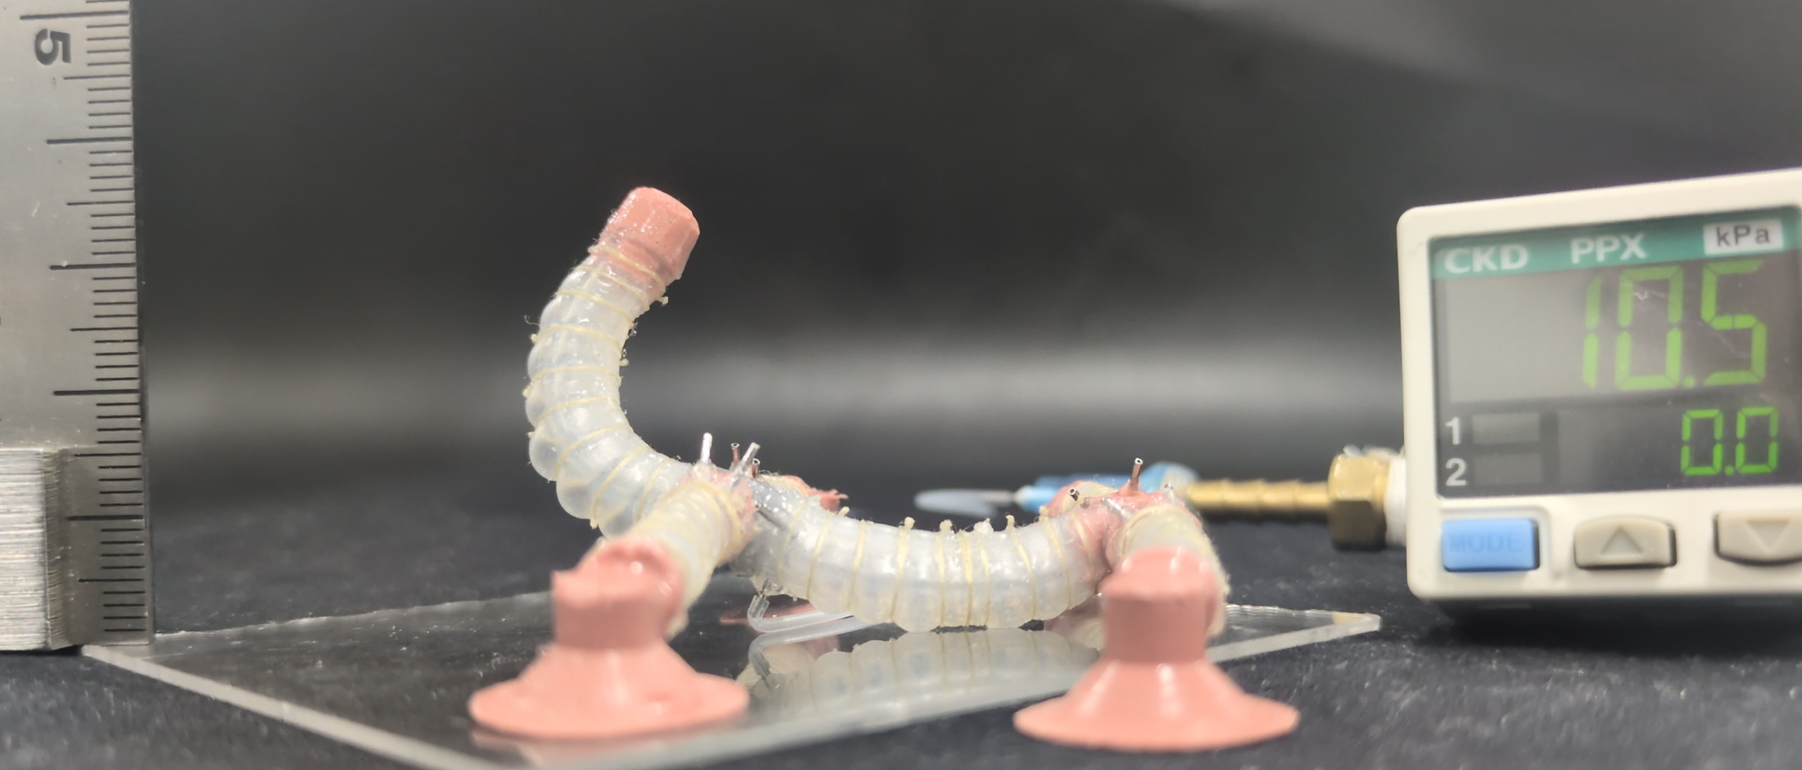
\includegraphics[width=0.95\columnwidth]{figures/Unonut10.5.png}
  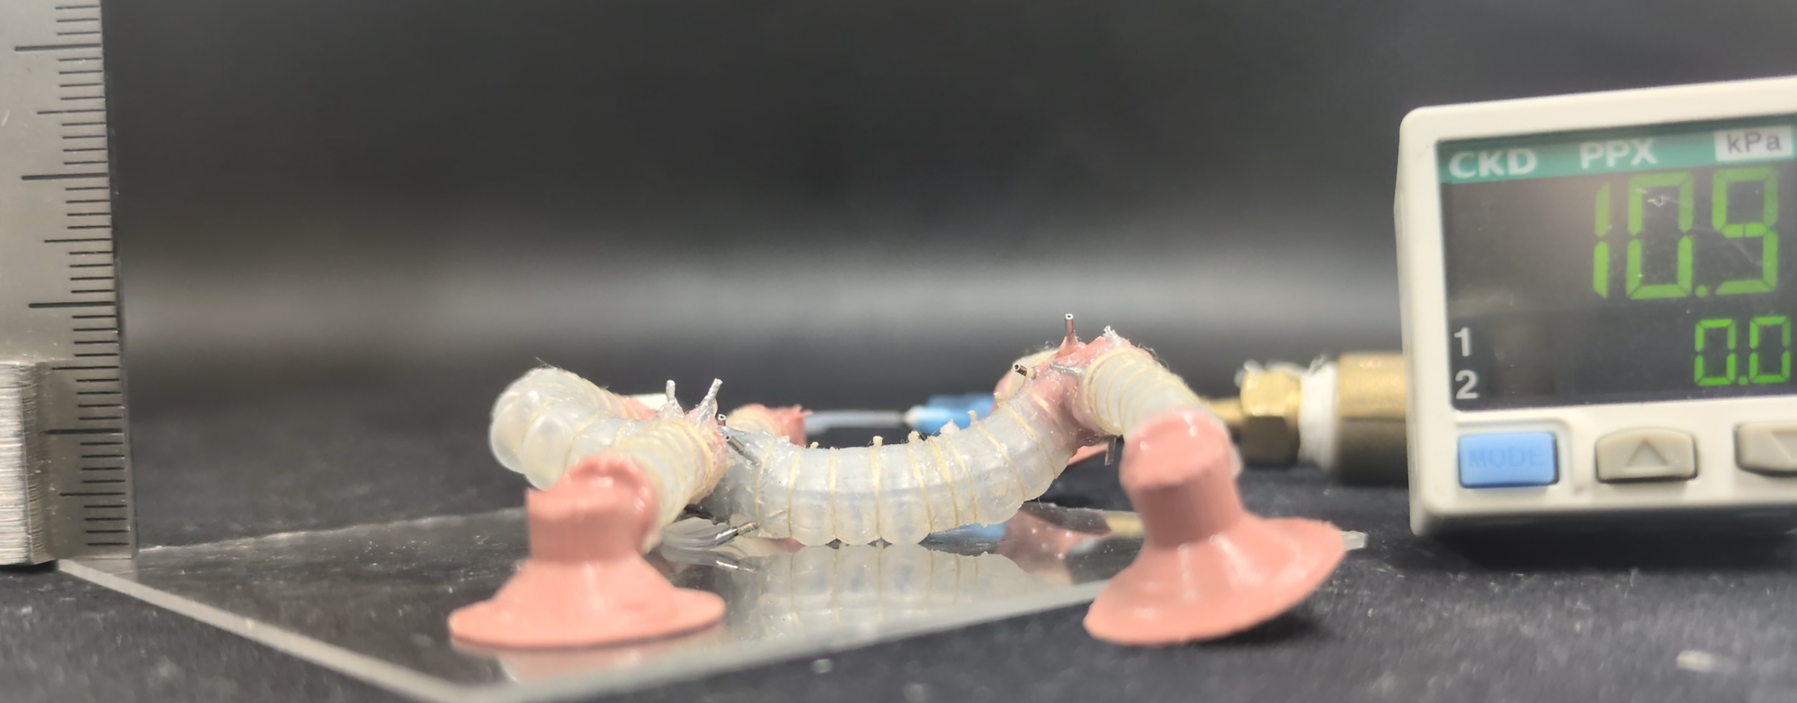
\includegraphics[width=0.95\columnwidth]{figures/Usmallnut10.9.png}
  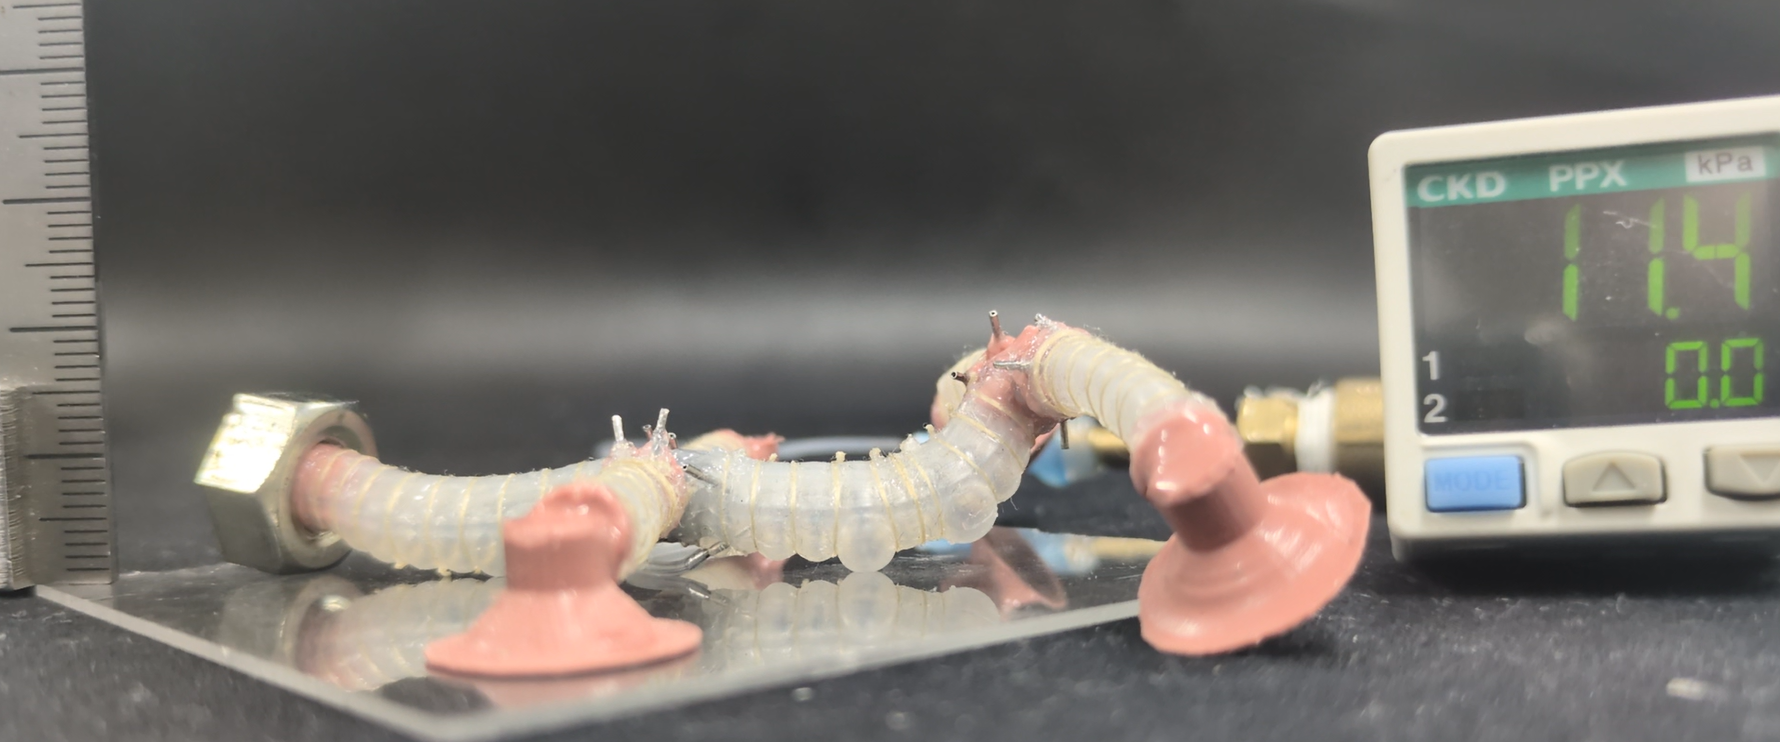
\includegraphics[width=0.95\columnwidth]{figures/Ubignut11.4.png}
  \caption{Side views of the assembled robot performing vertical U-shaped
  bending with the posterior suction-cup feet engaged. (a)~Without tip
  load, at 10.5~kPa. (b)~With a 2.0~g nut threaded onto the tip, at
  10.9~kPa. (c)~With a 5.7~g nut, at 11.4~kPa; the tip load in this case
  approximately equals the total robot mass of 5.8~g.}
  \label{fig:lizard-ubend-loads}
\end{figure}
